\newacronym{sujeitoa}{s.a.}{sujeito a}
\newacronym{nlp}{NLP}{\textit{Nonlinear Programming}}
\newacronym{mhe}{MHE}{Estimativa de Horizonte Móvel}

\chapter{Otimização}
\label{ch:otimizacao}

% =====================================================================================================
% ============================================= Section ===============================================
% =====================================================================================================
\section{O problema da otimização}
\label{sec:problema_da_otimizacao}

Segundo \citeonline{Haugen2018} normalmente problemas de otimização são apresentados
como problemas de minimização, como: "Encontre o valor ótimo de $x$ que minimize a
\textit{função objetivo} $f(x)$, levando em consideração qualquer restrição sobre $x$
ou em função de $x$. A solução ótima é indicada por
\simbolo{xopt}{$ x_{opt} $}{Valor ótimo de $x$ para minimizar $f(x)$}" \cite{Haugen2018}.

\citeonline{Haugen2018} ainda mostra que há várias formas de formular matematicamente
um problema de otimização (minimização), mas que, de forma geral, dado um modelo
matemático $M$, é possível representá-lo como a minimização de $x$ para uma função
$f(x)$, ou seja:

\begin{equation}
	\min_{x} f(x)
\end{equation}

sujeito a (também denotado por "\acrshort{sujeitoa}") restrições, que podem ser na forma de:

\begin{itemize}
\item Restrições de desigualdade:
	\begin{equation}
		\label{eq:min_restr_desigualdade}
		g(x) \leq 0
	\end{equation}
	onde $g$ pode ser uma função linear ou não-linear.
	
\item Restrições de igualdade:
	\begin{equation}
		\label{eq:min_restr_igualdade}
		h(x) = 0
	\end{equation}
	onde $h$ pode ser uma função linear ou não-linear de $x$.
	
\item Limites superiores e inferiores
	\begin{equation}
		\label{eq:min_limites}
		x_{li} \leq x \leq x_{ls}
	\end{equation}
	Onde $li$ e $ls$ indicam `limite inferior' e `limite superior', respectivamente.
\end{itemize}

Sendo que as equações \ref{eq:min_restr_desigualdade} e \ref{eq:min_restr_igualdade}
definem restrições na relação entre as variáveis de otimização, enquanto
\ref{eq:min_limites} define as regiões limites destas mesmas variáveis.

Existem diversos métodos para encontrar a solução ótima para um problema de otimização
e a seção a seguir irá mostrar exemplos e métodos numéricos simples para exemplificar,
em maiores detalhes, como um problema de minimização pode ser resolvido. No
\cref{ch:mpc} será feito uso das minimizações para compreender como o \acrshort{mpc}
calcula valores ótimos, dadas determinadas restrições em um dado horizonte de controle,
pois uma maior compreensão sobre problemas de minimização pode fazer grande diferença
no entendimento do controle \acrshort{mpc} em si.

% =====================================================================================================
% ============================================= Section ===============================================
% =====================================================================================================
\section{Algoritmos de otimização}
\label{sec:algoritmos_de_otimizacao}

% .....................................................................................................
% ............................................ Subsection .............................................
% .....................................................................................................
\subsection{Método de pesquisa em grade}
\label{subsec:metodo_pesquisa_em_grade}

O método apresentado nesta seção não é aplicável a praticamente nenhum problema real
devido a sua ineficiência computacional, porém ele ajuda a ilustrar o objetivo de
todo o método numérico voltado para minimização.

Este método consiste em testar todos os valores de todas as variáveis (em um conjunto
de dados definido) para verificar qual combinação minimiza a função objetivo, ou seja,
testar todos os valores possíveis para $x_1$, $x_2$, $x_3$, $...$, $x_n$ com o
objetivo de encontrar o \gls{xopt}, valor de $x$ que minimiza $f$.

% (Brincalepe) Mover o código de exemplo para o Apêndice			[ok]
No caso de um único $x$, um laço condicional simples poderia testar todos os valores da
função objetivo. Para ilustrar essa ideia, no \cref{ch:codigos_extras} o
código-fonte \ref{lst:grid_search_scalar}, em Python, mostra como a função $f(x)$ abaixo
poderia ser computada, caso o intervalo de teste de $x$ fosse igual 100, ou seja, $N = 100$.

\begin{equation}
	\label{eq:grid_search_scalar}
	f(x) = 0,00232x^4 - 0,111x^3 + 1,8x^2 - 11,6x + 34,4
\end{equation}

Sendo que:
\[	2 \leq x \leq 22 \]

O intervalo $N = 100$ indica que serão analisados 100 valores entre $2$ e $22$.

A \cref{fig:grid_search_scalar} foi construída a partir do código-fonte \ref{lst:grid_search_scalar},
sendo destacado em vermelho, o valor de $x$ onde a $f(x)$ apresentava seu menor valor.
Repare que o gráfico apresenta dois vales distintos: um deles é o já mencionado
destaque em vermelho, onde o valor $x$ é $18,76$ e outro onde $x$ vale
aproximadamente $5,5$. O vale do gráfico onde o valor de $x$ produz o menor valor
de $f(x)$ é conhecido como \textit{mínimo global}, todos os outros são
\textit{mínimos locais}, pois são os valores mínimos da função apenas para uma
região limitada.

Algoritmos que buscam encontrar o valor mínimo de uma função podem erroneamente
convergir para mínimos locais. O método de pesquisa em grade não é um desses
algoritmos, pois ao verificar todos os valores de $x$ ele sempre encontrará o
valor de $x$ que minimiza a função objetivo, porém nas próximas sessões serão
apresentados métodos que, apesar de serem mais eficientes computacionalmente,
podem tender para mínimos locais.
	
\begin{figure}
	\caption{Pesquisa em grade com número escalar}
	\begin{center}
		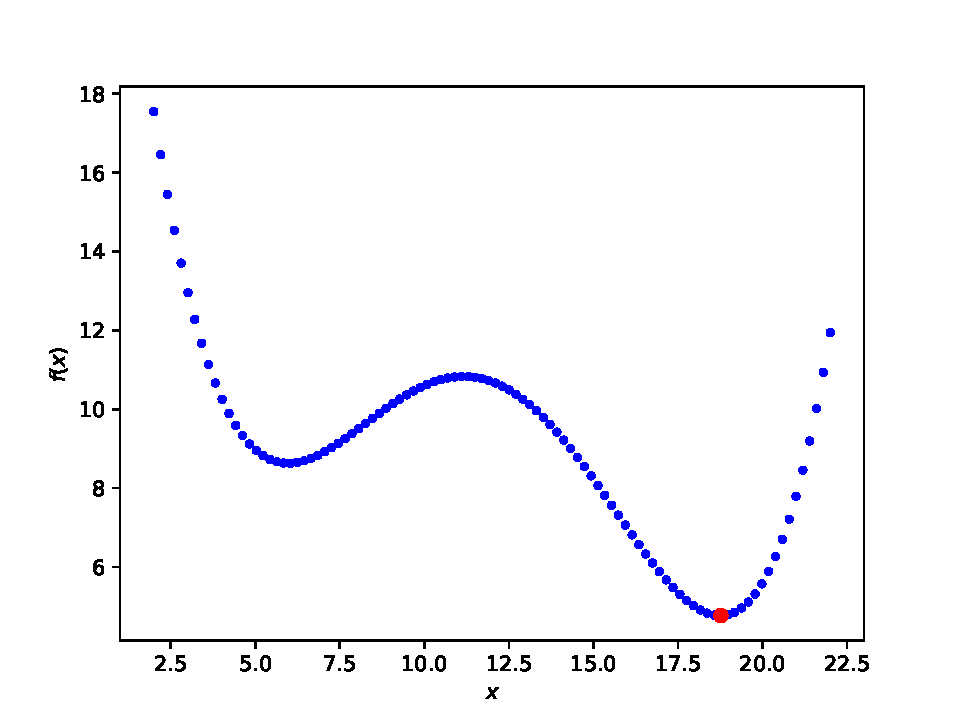
\includegraphics[width=0.8\textwidth]{./5_images/fig_grid_search_scalar.pdf} 
		\label{fig:grid_search_scalar}
	\end{center}
	\centering
	\makebox[\width]{Fonte: Autor, adaptado de \citeonline{Haugen2018}}
\end{figure}

Ainda neste método, casos onde há uma maior quantidade de variáveis ($x_1$, $x_2$, \dots)
deve-se utilizar laços aninhados para que a varredura de todas as possibilidades
possa ser feita. 

Como exemplo, minimizemos a \cref{eq:grid_search_vect_no_bounds}, sendo
$0 \leq x_1 \leq 2$ e $1 \leq x_2 \leq 3$.

\begin{equation}
	\label{eq:grid_search_vect_no_bounds}
	f(x) = (x_1 - 1)^2 + (x_2 - 2)^2 + 0,5
\end{equation}

Neste caso, de forma direta nota-se que
$f_{min} = 0,5$, $x_{1_{opt}} = 1$ e $x_{2_{opt}} = 2$.\footnote{
	O código-fonte em Python para este cálculo pode ser encontrado no							% Footnote
	\cref{ch:codigos_extras}, código-fonte \ref{lst:grid_search_vectorial}.}					% Footnote
Porém se a restrição da \cref{eq:grid_search_vect_bounds} for aplicada
novos valores são encontrados, descritos nas equações presentes em
\cref{eq:grid_search_vect_bounds_output}.

\begin{equation}
	\label{eq:grid_search_vect_bounds}
	f(x) = x_1 - x_2 + 1,5 \leq 0
\end{equation}

% \begin{subequations}
% 	\label{equ_grid_search_vect_bounds_output}
% 	\begin{align}
% 		f_{min} = 0,628 \\
% 		x_{1_{opt}} = 0,748 \\
% 		x_{2_{opt}} = 2,25
% 	\end{align}
% \end{subequations}

\begin{equation}
	\label{eq:grid_search_vect_bounds_output}
	\begin{aligned}
		f_{min} = 0,628 \\
		x_{1_{opt}} = 0,748 \\
		x_{2_{opt}} = 2,25
	\end{aligned}
\end{equation}

O motivo de os valores de $x_{1_{opt}}$ e de $x_{2_{opt}}$ serem diferentes quando a restrição
da \cref{eq:grid_search_vect_bounds} é aplicada pode ser visualmente observado nas figuras
\ref{fig:grid_search_vectorial_nobounds} e \ref{fig:grid_search_vectorial_withbounds} onde
elas mostram uma alteração do ponto mínimo da função custo (outra forma de chamarmos a função
objetivo) devido à redução do conjunto imagem de $f(x)$.

\begin{figure}[h]
    \centering
    \begin{minipage}{0.45\textwidth}
		\caption{Pesquisa em grade com duas variáveis e sem restrição}
        \centering
        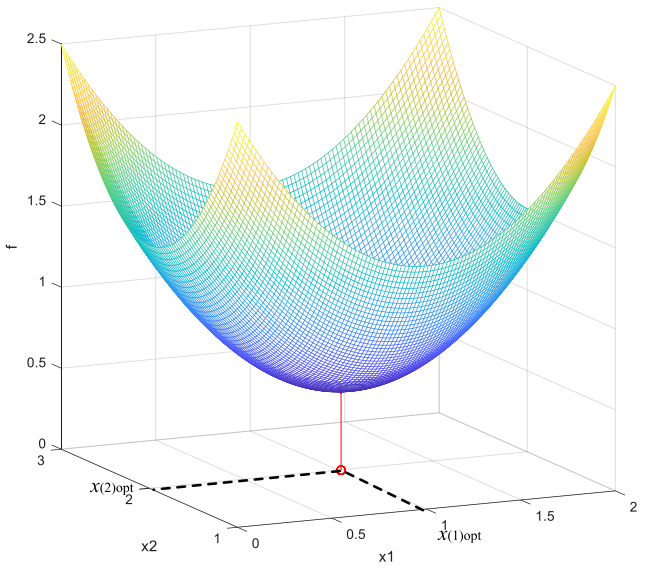
\includegraphics[width=0.9\textwidth]{./5_images/fig_grid_search_vectorial1.png} 
		\label{fig:grid_search_vectorial_nobounds}
		Fonte: \citeonline{Haugen2018}
    \end{minipage}\hfill
    \begin{minipage}{0.45\textwidth}
		\caption{Pesquisa em grade com duas variáveis e com restrição}  
        \centering
        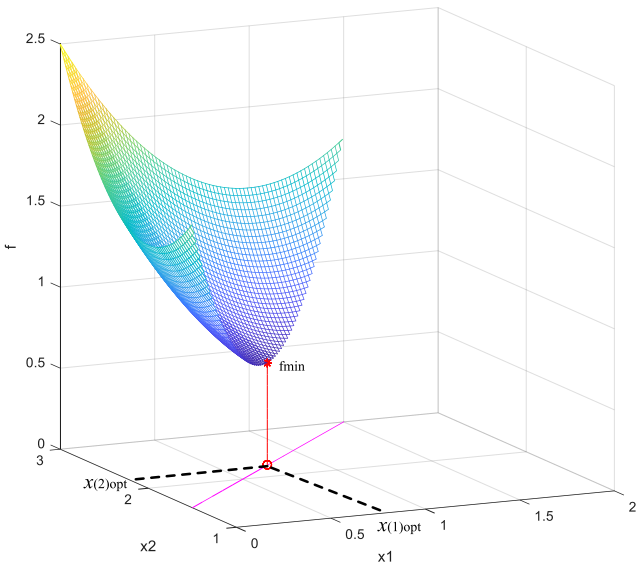
\includegraphics[width=0.9\textwidth]{./5_images/fig_grid_search_vectorial2.png} 
		\label{fig:grid_search_vectorial_withbounds}		      
		Fonte: \citeonline{Haugen2018}
	\end{minipage}
\end{figure}

% .....................................................................................................
% ............................................ Subsection .............................................
% .....................................................................................................
\subsection{Método de busca de descidas mais íngremes}
\label{subsec:metodo_descida_mais_ingreme}

Tal qual o método de pesquisa em grade, a maioria dos outros algoritmos de otimização
consiste em testar valores de $x$ e indicar qual deles retorna o menor $f(x)$,
porém, diferentemente do método anterior, a técnica apresentada nesta seção não testa
todos os valores possíveis de $x$, na realidade ela calcula o próximo valor de $x$ baseando-se
na derivada da função custo calculada no ponto $x$.

Exemplificando para um caso escalar podemos dizer que o próximo valor de $x$, isto é, $x_{k+1}$, será dado por:

\begin{subequations}
	\begin{align}
		x_{k+1} &= x_k + \Delta x_k		\label{eq:steepest_decent_xk1_a} \\ 
		\Delta x_k &= -K f'(x_k)		\label{eq:steepest_decent_xk1_b}
	\end{align}
\end{subequations}

\noindent
Onde: \\
$x_k$ = $x$ atual \\
$\Delta x_k$ = diferença entre $x_k$ e $x_{k+1}$ \\
$K$ = fator multiplicador do incremento \\
$f'(x_k)$ = derivada da função custo calculada em $x_k$
\newline

A derivada $f'(x_k)$ indica quão inclinada está a função custo no ponto $x_k$,
assim o fator $K$ determina o peso que essa inclinação terá para o cálculo do
próximo valor de $x$.

A \cref{fig:steepest_decent_slope} mostra graficamente a influência da derivada
da função custo na amplitude de $\Delta x_k$ entre iterações. Na figura vemos
a derivada aplicada sobre dois pontos distintos, $x_a$ e $x_b$, e podemos notar
que $f'(x_b)$ será menor que $f'(x_a)$ uma vez que $x_b$ está mais próximo ao 
ponto mínimo de $f'$.

\begin{figure}
	\caption{Influência de $f'(x_k)$ no cálculo de $x_{k+1}$ no método de descidas mais íngremes}
	\begin{center}
		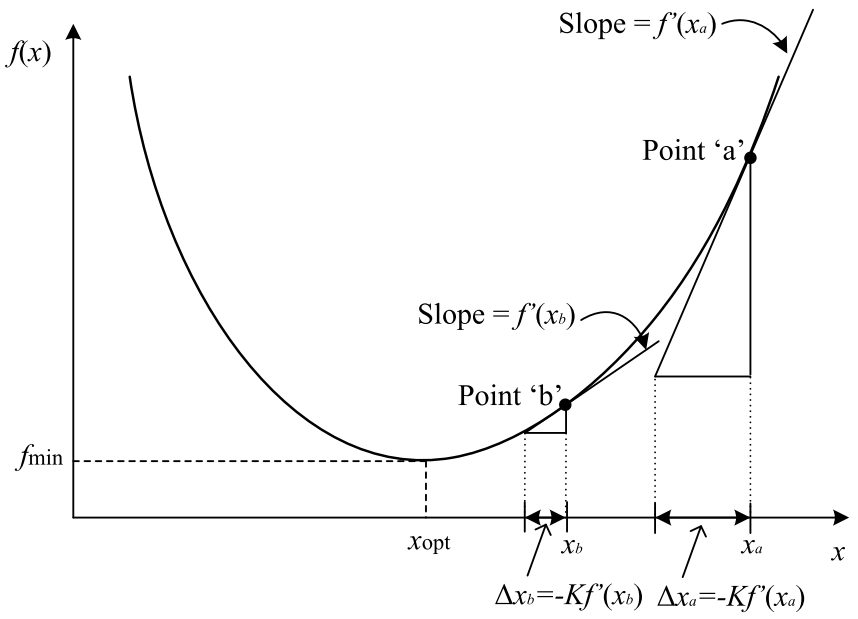
\includegraphics[width=0.75\textwidth]{./5_images/fig_steepest_decent_slope.png} 
		\label{fig:steepest_decent_slope}
	\end{center}
	\centering
	\makebox[\width]{Fonte: \citeonline{Haugen2018}}
\end{figure}
% TODO: Traduzir imagem

Como indicado na \cref{eq:steepest_decent_xk1_a}, o cálculo de $x_{k+1}$ depende
de $x_k$, ou seja, o valor do próximo $x$ calculado depende do $x$ anterior. Para
o cálculo de $x_1$ é necessário fazer uma estimativa de $x_0$. A maior parte das
funções de otimização requerem como argumento um valor de $x_0$ estimado, pois é
a partir dele que serão iniciadas as buscas até o ponto mínimo da função.

As mesmas equações se aplicam para casos onde $\mathrm{x}$ é um vetor, com a diferença que
ao invés de calcularmos a derivada sobre o ponto $\mathrm{x}_k$, calculamos o gradiente
do vetor $\mathrm{x}_k$, tal qual vemos na \cref{eq:steepest_decent_xk1_vectorial_b}.

\begin{subequations}
	\begin{align}
		\mathrm{x}_{k+1} &= \mathrm{x}_k + \Delta \mathrm{x}_k			\label{eq:steepest_decent_xk1_vectorial_a} \\ 
		\Delta \mathrm{x}_k &= \mathrm{-K} \nabla f(\mathrm{x}_k)		\label{eq:steepest_decent_xk1_vectorial_b}
	\end{align}
\end{subequations}

\noindent
Sendo que: \\
% \[
\begin{align*}
	\mathrm{x}_k &= 					% TODO: Ajustar a esquerda
	\begin{bmatrix}
		x(1)_{k} \\
		x(2)_{k} \\
		\vdots \\
		x(n)_{k}
	\end{bmatrix} \\
	% \]
	\mathrm{K} &= \text{fator multiplicador do incremento} \\
	\nabla f(\mathrm{x}_k) &= \text{gradiente da função custo calculada em } \mathrm{x}_k
\end{align*}
\newline

Além de requerer um valor estimado para $x_0$, este método também apresenta um
critério de parada, isto é, uma condição que quando alcançada irá parar o laço de
iterações por já ter encontrado o $f_{min}$. Este critério é dado pela \cref{eq:steepest_descent_stop}
e ao alcançá-la então $x_{opt}$ será $x_{k+1}$.

\begin{equation}
	\label{eq:steepest_descent_stop}
	|f(x_{k+1})-f(x_k)| \leq df
\end{equation}

\noindent
Onde: \\
$df$ = Valor do critério de parada (ex. 0,00001)
\newline

O código-fonte \ref{lst:steepest_descent_vectorial} exemplifica a utilização deste método
para as equações descritas em \ref{eq:steepest_decent_vectorial_example}.

\begin{subequations}
	\label{eq:steepest_decent_vectorial_example}
	\begin{gather}
		\min_{x} f(x) \\ 
		f(\mathrm{x}) = [x(1) - 1]^2 + [x(2) - 2]^2 + 0,5		\label{eq:steepest_decent_vectorial_example_fobj} \\
		|f(\mathrm{x}_{k+1}) - f(\mathrm{x}_k)| \leq df 		\label{eq:steepest_decent_vectorial_example_stop} \\
		df = 10^{-4}											\label{eq:steepest_decent_vectorial_example_df}
	\end{gather}
\end{subequations}

\lstinputlisting[	
	caption={Busca por descidas mais íngremes},
	captionpos=t,
	label={lst:steepest_descent_vectorial},
	language=Python,
	style=Python_lang]
	{./4_Codes/steepest_descent_vectorial.py}
	\begin{center}
		\makebox[\width]{Fonte: Autor, adaptado de \citeonline{Haugen2018}}
	\end{center}

Um problema conhecido deste método é o fato de ele poder não distinguir entre
mínimos locais e mínimos globais fazendo com que o valor que é apontado como
$f_{min}$ possa ser na verdade apenas um mínimo local. O valor de $x_0$
estimado tem impacto direto neste resultado, pois como este método
inicia o cálculo da derivada de $f(x)$ no ponto $x_0$, então as iterações seguintes
dependerão exclusivamente da iteração anterior, fazendo assim uma convergência para
o mínimo mais próximo, seja ele local ou global. As
\cref{fig:steepest_descent_global_minimum,fig:steepest_descent_local_minimum}
mostram mais detalhadamente esta diferença.

\begin{figure}[h]
    \centering
    \begin{minipage}{0.47\textwidth}
		\caption{Método de descida mais íngrime convergindo para mínimo global}
        \centering
        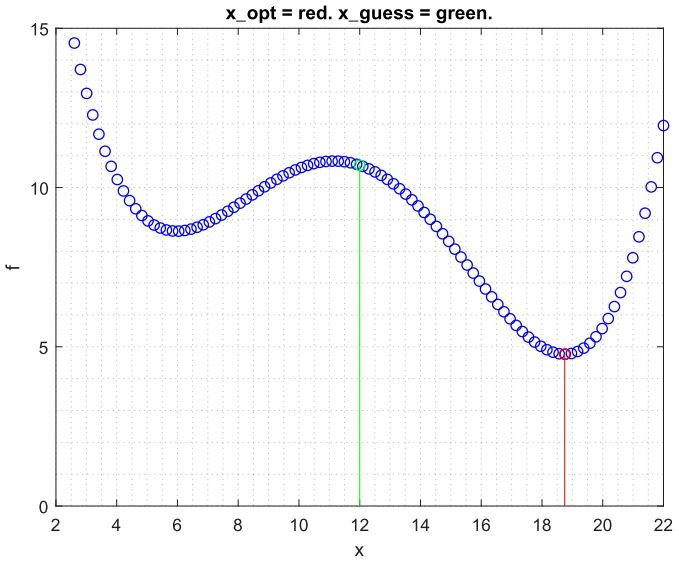
\includegraphics[width=0.9\textwidth]{./5_images/steepest_descent_global_minimum.png} 
		\label{fig:steepest_descent_global_minimum}
		Fonte: \citeonline{Haugen2018}
    \end{minipage}\hfill
    \begin{minipage}{0.47\textwidth}
		\caption{Método de descida mais íngrime convergindo para mínimo local}  
        \centering
        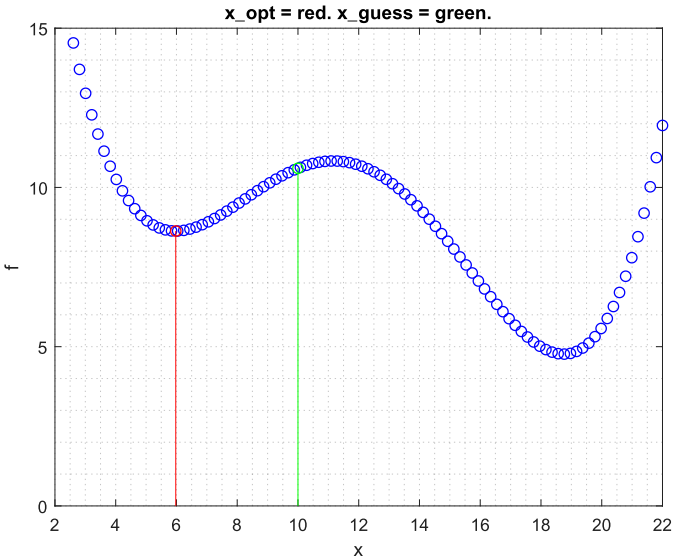
\includegraphics[width=0.9\textwidth]{./5_images/steepest_descent_local_minimum.png} 
		\label{fig:steepest_descent_local_minimum}		      
		Fonte: \citeonline{Haugen2018}
	\end{minipage}
\end{figure}

As \cref{fig:steepest_descent_global_minimum,fig:steepest_descent_local_minimum}
apresentam a mesma função custo, porém na \cref{fig:steepest_descent_global_minimum}
$x_0 = 12$, e as derivadas consecutivas a partir desde valor convergem para o
mínimo global; já na \cref{fig:steepest_descent_local_minimum} estimasse $x_0 = 10$
resultando em um $f_{min}$ completamente diferente, convergindo para um mínimo local.
Em ambas as figuras a linha verde indica o valor de $x_0$ e a linha vermelha indica
o $f_{min}$ quando o critério de parada é atingido.

% .....................................................................................................
% ............................................ Subsection .............................................
% .....................................................................................................
\subsection{Otimizadores de programação não-linear (NLP)}
\label{subsec:otimizadores_nlp}

Muitos métodos de otimização não suportam restrições como as descritas nas
\cref{eq:min_restr_desigualdade,eq:min_restr_igualdade}, este é, por exemplo, o caso
do método de busca de descidas mais íngremes, porém outros métodos podem levar esse tipo
de restrição em conta, e estes são conhecidos como Otimizadores de Programação não-linear
(do inglês \acrlong{nlp}, ou simplesmente \acrshort{nlp}) \cite{Haugen2018}.

Otimizadores \acrshort{nlp} são úteis quando há a necessidade de métodos de otimização
que sejam mais robustos e mais flexíveis do que técnicas mais simples, como o método
de busca de Newton, ou aqueles apresentados nas sessões anteriores deste trabalho e por
isso muitos softwares como o \acrshort{matlab} e bibliotecas da
linguagem Python dispõem de ferramentas para cálculo de métodos \acrshort{nlp}. No
\acrshort{matlab} o \textit{Optimization Toolbox}\textsuperscript{TM}\footnote{
	O \acrshort{matlab} \textit{Optimization Toolbox}\textsuperscript{TM} é um conjunto					% footnote
	de ferramentas de otimização que provê funções para encontrar parâmetros que minimizem				% footnote
	ou maximizem objetivos, satisfazendo as condições limites. Mais detalhes em							% footnote
	\href{www.mathworks.com/products/optimization.html}{www.mathworks.com/products/optimization.html}	% footnote
} possui a função \textit{fmincon} enquanto no Python podemos encontrar a função
\textit{scipy.optimize.minimize} na biblioteca \textit{SciPy}\footnote{
	A biblioteca \textit{SciPy} (do inglês \textit{SciPy Library}) faz parte do conjunto de				% footnote
	soluções do programa \textit{SciPy}. A biblioteca \textit{SciPy} fornece uma interface				% footnote
	de usuário amigável para cálculos de integração numérica, interpolação, otimização,					% footnote
	algebra linear, estatística, entre outros. Mais detalhes em 										% footnote
	\href{www.scipy.org/scipylib/index.html}{www.scipy.org/scipylib/index.html}							% footnote
}.

Os autores \citeonline{Haugen2018}, \citeonline{Ruggiero2000} apresentam em maiores detalhes
os métodos descritos nesta seção, além de muitos outros.

A documentação referente as funções fmincon e scipy.optimize.minimize encontram-se, respectivamente,
no \crefanexo{ch:documentacao_de_funcoes}, seções \ref{sec:fmincon} e \ref{sec:scipy_optimize_minimize}.
% (Brincalepe): Adicionar documentação sobre essas funções em um anexo			[ok]

% =====================================================================================================
% ============================================= Section ===============================================
% =====================================================================================================
\section{Algumas aplicações de otimização}
\label{sec:aplicacoes_de_otimizacao}

% .....................................................................................................
% ............................................ Subsection .............................................
% .....................................................................................................
\subsection{Estimação de parâmetros}
\label{subsec:estimacao_de_parametros}

Estimar parâmetros de um modelo pode ser uma das inúmeras aplicações dos métodos de otimização.
Segundo \citeonline{Haugen2018} um problema de estimação de parâmetros pode ser formulado
como mostrado na \cref{eq:parameter_estimation}, visando encontrar os parâmetros que
apresentem menor diferença entre o sistema real e o modelo sendo avaliado.
A comparação o sistema real e o virtual é feita através do acúmulo da diferença das saídas dos
dois sistemas elevada ao quadrado ao longo de $N$ iterações.

\begin{equation}
	\label{eq:parameter_estimation}
	\min_{P} \sum_{k=1}^{N} e(k)^2
\end{equation}

\noindent
Onde: \\
$P$ = vetor de parâmetros a ser estimado. Sendo $ P = [p(1), p(2), ..., p(r)]^T $ \\
$e$ = erro de predição. Sendo $ e = y_{medido} - y_{modelo} $ \\
$ y_{medido} $ = medição da saída do sistema real \\
$ y_{modelo} $ = cálculo da saída do modelo simulado \\
$ N $ = quantidade de amostras
\newline

O diagrama de blocos apresentado na \cref{fig:parameter_estimation} apresenta de forma
visual a comparação entre o sistema real e o modelo matemático.

\begin{figure}
	\caption{Diagrama de blocos do quadrado da diferença entre o sistema real e o modelo}
	\begin{center}
		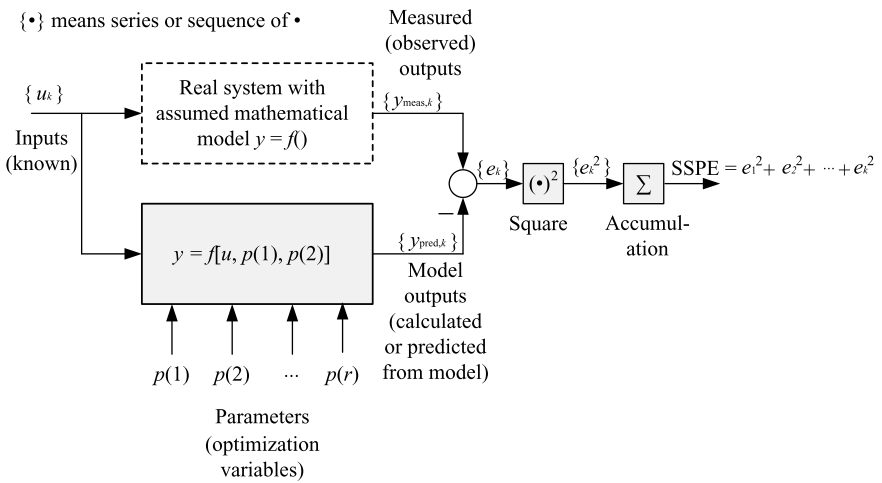
\includegraphics[width=0.75\textwidth]{./5_images/fig_parameter_estimation.png} 
		\label{fig:parameter_estimation}
	\end{center}
	\centering
	\makebox[\width]{Fonte: \citeonline{Haugen2018}}
\end{figure}
% TODO: Traduzir imagem

Para estimar os parâmetros $P$ de um dado modelo é necessário dividir os dados amostrais
$N$ em dois grupos: um deles destinado a adaptação do modelo, ou seja, encontrar o vetor $P$
que minimize a função custo, e o outro grupo destinado a validação, isto é, verificar se os
parâmetros encontrados durante a adaptação realmente é válido e preciso.

Quando dispomos de dados previamente coletados do sistema é possível fazer uma \textit{estimação
em batelada} (também conhecida como \textit{offline} \cite{Bolognani2009}), onde as fases de coleta e
estimação acontecem em momentos distintos. Já a \textit{estimação recursiva} (ou \textit{online}
\cite{Stadler2011}) ocorre quando a coleta dos dados e a estimação dos parâmetros acontece ao mesmo tempo.
A \cref{subsec:moving_horizon_estimation} descreve com mais detalhes a
\acrlong{mhe} (do inglês, \textit{Moving Horizon Estimation}, ou simplesmente \acrshort{mhe}), que,
assim como o filtro de Kalman, pode ser utilizado como estimador de parâmetros recursivo.
% TODO: (Brincalepe) Filtro de Kalman será detalhado?

% .....................................................................................................
% ............................................ Subsection .............................................
% .....................................................................................................
\subsection{\acrlong{mhe} (\acrshort{mhe})}
\label{subsec:moving_horizon_estimation}

O método conhecido como \acrlong{mhe} é um método estimador recursivo de parâmetros
que utiliza as medições atuais, anteriores e também as entradas do sistema sob um horizonte
fixo de tempo para calcular o estado atual do sistema, assim como ilustrado na \cref{fig:mhe}.
% TODO: (Brincalepe) Incluir citação

\begin{figure}[h]
	\caption{Horizonte de tempo analisado pelo método \acrlong{mhe}}
	\begin{center}
		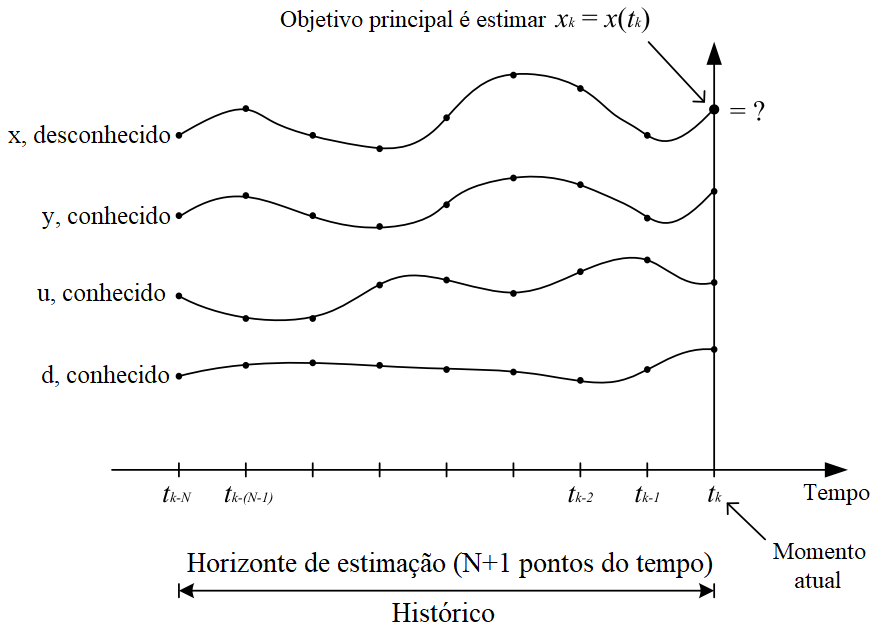
\includegraphics[width=0.75\textwidth]{./5_images/fig_mhe.png} 
		\label{fig:mhe}
	\end{center}
	\centering
	\makebox[\width]{Fonte: \citeonline{Haugen2018}}
\end{figure}
% TODO: Traduzir imagem

O modelo de espaço de estado que descreve o sistema pode ser descrito como indicado na
\cref{eq:mhe_main}.

\begin{subequations}
	\label{eq:mhe_main}
	\begin{gather}
		\mathrm{x}_{k+1} = \mathrm{f}(\mathrm{x}_k, \cdots) + \mathrm{w}_k		\label{eq:mhe_main_a} \\
		\mathrm{y}_k = \mathrm{g}(\mathrm{x}_k, \cdots) + \mathrm{v}_k			\label{eq:mhe_main_b}
	\end{gather}
\end{subequations}

\noindent
Onde: 
\begin{itemize}
	\item $\mathrm{x}$ é o vetor de estado a ser estimado.
		\begin{equation}
			\mathrm{x}_k =
			\begin{bmatrix}
				x(1)_{k} \\
				x(2)_{k} \\
				\vdots \\
				x(n)_{k}
			\end{bmatrix}
		\end{equation}
		
	\item $\mathrm{f}$ é um vetor de $n$ funções lineares ou não-lineares de $x_k$
		\begin{equation}
			\mathrm{f} =
			\begin{bmatrix}
				f_1(x_k, \cdots) \\
				f_2(x_k, \cdots) \\
				\vdots \\
				f_n(x_k, \cdots) \\
			\end{bmatrix}
		\end{equation}
		Os pontos representam possíveis argumentos adicionais de $f$ como a variável de
		controle ($u_k$), os distúrbios do processo ($d_k$), e os parâmetros ($p$).
		
	\item $\mathrm{w}_k$ representa os distúrbios não conhecidos ou não modelados do processo
			agindo sobre o estado, no instante $k$. Não é necessário assumir nenhuma propriedade
			estatística particular para este distúrbio, porém é sensato assumir um ruído, como o
			ruído branco, com uma matriz de covariância $Q$, assim como utilizado no filtro de
			Kalman. A matriz $Q$ será apresentada com mais detalhes a seguir.
	
	\item $\mathrm{y}$ é o vetor de saída com $m$ elementos.
	
	\item $\mathrm{g}$ é um vetor de $m$ funções lineares ou não-lineares de $\mathrm{x}_k$, onde os pontos
			também representam possíveis argumentos adicionais.

	\item $\mathrm{v}_k$ representa o erro medido, e, assim como $\mathrm{w}_k$, não necessita
			assumir nenhuma propriedade estatística particular, porém também é comum utilizar
			um ruído branco, com uma matriz de covariância $R$, também melhor apresentada a
			seguir.
	
\end{itemize}

O problema de otimização do \acrshort{mhe} pode ser descrito como na \cref{eq:mhe_minimization}.
% TODO: (Brincalepe) Detalhar Norma2

\begin{equation}
	\label{eq:mhe_minimization}
	\min_{X} \sum_{i=k-N}^{k-1} \Vert x_{i+1} - f(x_i, \cdots) \Vert^2_{Q^{-1}} + 
			\sum_{i=k-N}^{k} \Vert y_i - g(x_i, \cdots) \Vert^2_{R^{-1}}
\end{equation}

Sendo que $X$ é a matriz contendo o estado a cada ponto do horizonte de estimação:
\begin{equation}
	\begin{aligned}
		X &= [\mathrm{x}_{k-N}, \mathrm{x}_{k-N-1}, \cdots, \mathrm{x}_{k-1}, \mathrm{x}_k] \\
		&=
		\begin{bmatrix}
			x(1)_{k-N} & x(1)_{k-(n-1)} & \cdots & x(1)_{k-1} & x(1)_k		\\
			x(2)_{k-N} & x(2)_{k-(n-1)} & \cdots & x(2)_{k-1} & x(2)_k		\\
			\vdots & \vdots & \ddots & \vdots & \vdots						\\
			x(n)_{k-N} & x(n)_{k-(n-1)} & \cdots & x(n)_{k-1} & x(n)_k	
		\end{bmatrix}
	\end{aligned}
\end{equation}

E com base na \cref{eq:mhe_main} este problema também pode ser descrito como:

\begin{equation}
	\label{eq:mhe_minimization2}
	\min_{X} \sum_{i=k-N}^{k-1} \Vert \mathrm{w}_i \Vert^2_{Q^{-1}} + 
			\sum_{i=k-N}^{k} \Vert \mathrm{v}_i \Vert^2_{R^{-1}}
\end{equation}

Ou mesmo:

\begin{equation}
	\label{eq:mhe_minimization3}
	\min_{X} \sum_{i=k-N}^{k-1} \mathrm{w}^T_i Q^{-1} \mathrm{w}_i + 
			\sum_{i=k-N}^{k} \mathrm{v}^T_i R^{-1} \mathrm{v}_i
\end{equation}

\noindent
Onde: 
\begin{itemize}
	\item $\mathrm{w}_i$ é o vetor de distúrbio do processo.
		\begin{equation}
			\mathrm{w}_i =
			\begin{bmatrix}
				w(1)_{i} \\
				w(2)_{i} \\
				\vdots \\
				w(n)_{i}
			\end{bmatrix}
		\end{equation}
		
	\item $\mathrm{v}_i$ é um vetor de erros de medição.
		\begin{equation}
			\mathrm{v}_i =
			\begin{bmatrix}
				v(1)_{i} \\
				v(2)_{i} \\
				\vdots \\
				v(m)_{i}
			\end{bmatrix}
		\end{equation}
		
	\item $\mathrm{Q}^{-1}$ é a matriz de ponderação de $\mathrm{w}_i$
		\begin{equation}
			\mathrm{Q}^{-1} =
			\begin{bmatrix}
				\frac{1}{Q_{11}} & \cdots & 0 \\
				\vdots & \ddots & \vdots \\
				0 & \cdots & \frac{1}{Q_{nn}}
			\end{bmatrix}
		\end{equation}
		Assumindo que $w$ é aleatório, então $Q$ pode ser interpretado como a inversa
		da matriz de covariância do distúrbio do processo.

	\item $\mathrm{R}^{-1}$ é a matriz de ponderação de $\mathrm{v}_i$
		\begin{equation}
			\mathrm{R}^{-1} =
			\begin{bmatrix}
				\frac{1}{R_{11}} & \cdots & 0 \\
				\vdots & \ddots & \vdots \\
				0 & \cdots & \frac{1}{R_{nn}}
			\end{bmatrix}
		\end{equation}
		Assumindo que $v$ é aleatório, então $R$ pode ser interpretado como a inversa
		da matriz de covariância do distúrbio do processo.
	
\end{itemize}

Desta forma a \cref{eq:mhe_minimization3} pode ser reescrita como:

\begin{equation}
	\label{eq:mhe_minimization4}
	\min_{X} \sum_{i=k-N}^{k-1} \begin{bmatrix} \frac{w(1)^2_i}{Q_{11}} + \cdots + \frac{w(n)^2_i}{Q_{nn}} \end{bmatrix} + 
			\sum_{i=k-N}^{k} \begin{bmatrix} \frac{v(1)^2_i}{R_{11}} + \cdots + \frac{v(n)^2_i}{R_{mm}} \end{bmatrix}
\end{equation}

Resumidamente observa-se que o \acrshort{mhe} utiliza as medições (minimizando a influência dos
erros de medição) e o modelo (minimizando os erros de modelo) para calcular o estado estimado.

% -----------------------------------------------------------------------------------------------------
% ------------------------------------------- Subsubsection -------------------------------------------
% -----------------------------------------------------------------------------------------------------
\subsubsection{Exemplo}
\label{subsubsec:mhe_example}

A \cref{fig:mhe_example} mostra o gráfico de uma simulação executada através do código-fonte \ref{lst:mhe_example}
exemplificando a aplicação da técnica \acrlong{mhe} para o modelo simplificado da velocidade de um motor de corrente
contínua.

O modelo dinâmico do motor é apresentado na \cref{eq:motor_dynamics} e sua representação no espaço de estados
na \cref{eq:motor_dynamics_ss}, sendo que esta é a representação utilizada no código-fonte \ref{lst:mhe_example}.

\begin{equation}
	\label{eq:motor_dynamics}
	T \dot{S} = -S + Ku + L
\end{equation}

\noindent
Onde: 												\\
$u$ = sinal de controle (tensão aplicada ao motor)	\\
$S$ = sinal medido (velocidade do motor)			\\
$K$ = ganho 										\\
$T$ = constante de tempo 							\\
$L$ = carga

\begin{subequations}
	\label{eq:motor_dynamics_ss}
	\begin{align}
		\dot{x}(1) &= x(2) 					\\
		\dot{x}(2) &= [-x(2) + Ku] / T + d	\\
		y &= x(1)
	\end{align}
\end{subequations}

\lstinputlisting[	
	caption={Exemplo do método \acrlong{mhe}},
	captionpos=t,
	label={lst:mhe_example},
	language=Python,
	style=Python_lang]
	{./4_Codes/mhe_example.py}
	\begin{center}
		\makebox[\width]{Fonte: Autor, adaptado de \citeonline{Haugen2018}}
	\end{center}
	
\begin{figure}[h]
	\caption{Simulação utilizando \acrlong{mhe}}
	\begin{center}
		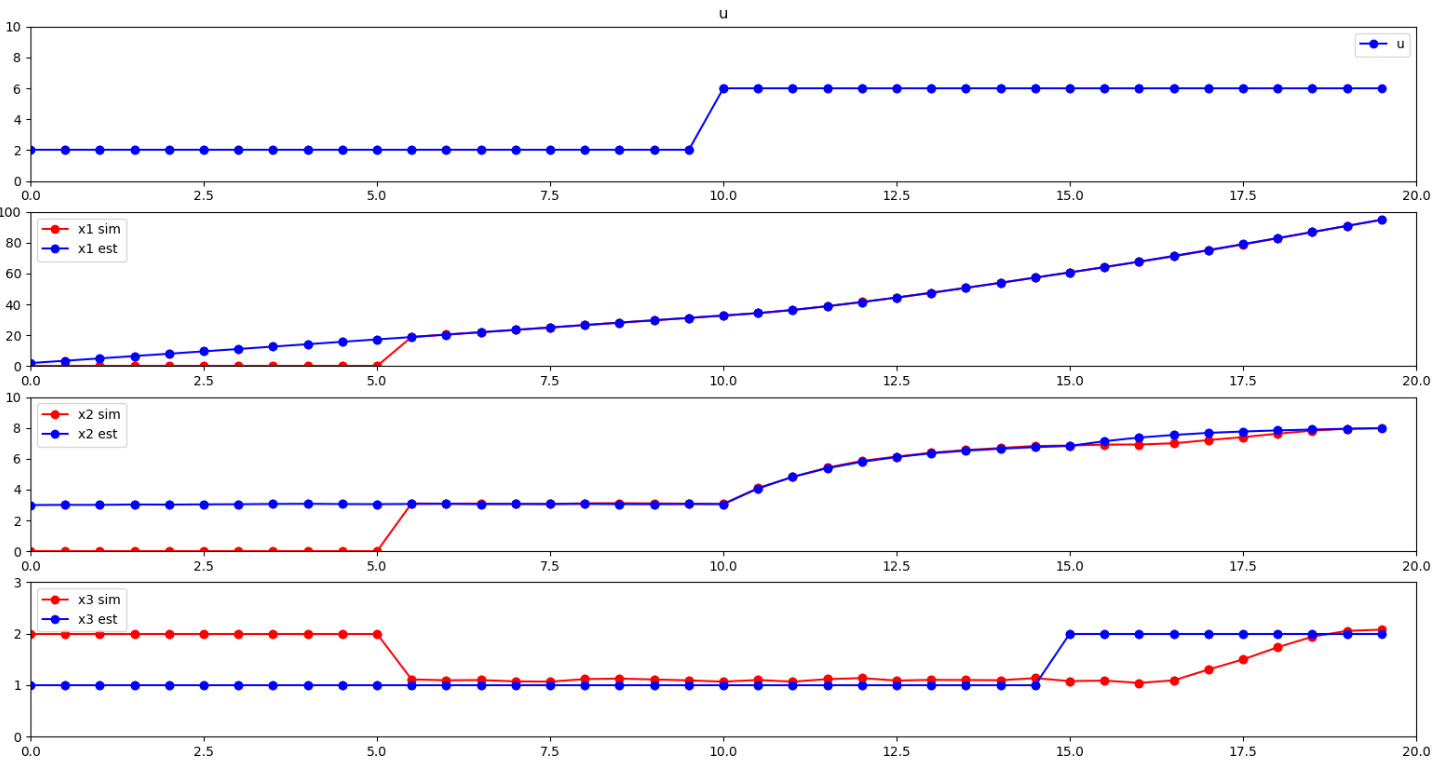
\includegraphics[width=1\textwidth]{./5_images/fig_mhe_example.png} 
		\label{fig:mhe_example}
	\end{center}
	\centering
	\makebox[\width]{Fonte: Autor, adaptado de \citeonline{Haugen2018}}
\end{figure}
% TODO: (Brincalepe) Interpretar imagem